\documentclass{article}
\usepackage[utf8]{inputenc}
\usepackage{graphicx}
\usepackage[table,xcdraw]{xcolor}


\title{My first document}
\author{Haruyaa}

\begin{document}
	\maketitle
	\section*{Project Name:}
		Predicting floods in coastal regions as a direct consequence of deforestation.
	\section*{Introduction/Motivation}
		The degree and scale of flood hazards have increased massively with the changing climate in the last decades, and large-		scale flash floods bring fast-moving and rapid-rising water with force, resulting in tremendous life and property losses as well as social disruption worldwide. Cutting of mangroves and trees in coastal regions and river plains for land development has led to decreasing water retention and increasing surface runoff which in turn increases the probability of flash floods. Thus, flood prediction and flood control are important issues for policy makers and designers. To mimic the complex mathematical expressions of physical processes of floods, during the past two decades, machine learning (ML) methods and Artificial intelligence (AI) contributed highly in the advancement of prediction systems providing better performance and cost-effective solutions.
Flooding in coastal areas depends on factors such as rainfall, sea tides, bank heights, man-made structures like embankments and reservoirs and mangroves and forest cover. Our proposed system will identify food prone regions and link flooding to deforestation in the area to allow sustainable growth in the future by giving afforestation as a solution to mitigate effects of floods.   
	\section*{Market Research / Literature Survey:}
		Many ML algorithms, e.g., artificial neural networks (ANNs), neuro-fuzzy, support vector machine (SVM), and support vector regression (SVR), have been employed for flood-prediction and were reported as effective for both short-term and long-term flood forecast. 
The performance of any Machine Learning method in flood prediction can be improved through hybridization with other ML methods. Such applications provide more robust and efficient models that can effectively learn complex flood systems in an adaptive manner. 
	\section{Hardware requirements:}
		None
\section*{Software requirements:}
\begin{table}[]
\begin{tabular}{|l|l|l|l|}
\hline
\rowcolor[HTML]{A6DFA6} 
\textbf{Service Type}          & \textbf{Custom Name} & \textbf{Region} & \textbf{Description}                                                                                                                                                                                                                                                                                            \\ \hline
Azure Machine Learning Service &                      & Southeast Asia  & D3 v2: 4 vCPU(s), 14GB RAM, $0.316/hour x 300 Hours, Pay as you go. Machine Learning Service Surcharge $0.040 x 4 core(s) x 300 Hours. Model Deployment with AKS.                                                                                                                                               \\ \hline
Virtual Machines               &                      & Southeast Asia  & \begin{tabular}[c]{@{}l@{}}D4 v3 (4 vCPU(s), 16 GB RAM), 100 GB Temporary Storage, \$0.434/hour. 1 x 300 Hours, Pay as you go.\\ Managed OS Disk - S4, Standard HDD, 32 GiB, 1 Disk, 100 transaction units\end{tabular}                                                                                         \\ \hline
Azure Open Datasets            &                      & West US         & Free                                                                                                                                                                                                                                                                                                            \\ \hline
Machine Learning Studio        &                      & Southeast Asia  & Workspace, Free                                                                                                                                                                                                                                                                                                 \\ \hline
Azure Cosmos DB                &                      & Southeast Asia  & 0 GB Storage; Single Region Write, Pay as you go, 4 x 100 RUs x 300 Hours x \$0.08/Hour.                                                                                                                                                                                                                        \\ \hline
Azure SQL Database             &                      & West India      & \begin{tabular}[c]{@{}l@{}}Managed Instance, vCore Purchase Model, LRS,\\ General Purpose Tier, Gen 4,  8 vCore\\ instance(s) x 300 Hours, 1 x 32 GB Storage\end{tabular}                                                                                                                                       \\ \hline
Cognitive Services             &                      & Southeast Asia  & \begin{tabular}[c]{@{}l@{}}Computer Vision: Free tier, 5000 included transactions.\\ Custom Vision: Free tier,  5,000 training images free per project, 10,000 predictions per month\end{tabular}                                                                                                               \\ \hline
Power BI Embedded              &                      & Southeast Asia  & Node type: A1, 1 Virtual Core(s), 3GB RAM, 1-300 Peak renders/hour. 1 Node(s) x 300 Hours,                                                                                                                                                                                                                      \\ \hline
Storage Accounts               &                      & West India      & \begin{tabular}[c]{@{}l@{}}Block Blob Storage, General Purpose V2, LRS\\ Redundancy, Hot Access Tier, 1,000 GB\\ Capacity, 100,000 Write operations, 100,000\\ List and Create Container Operations, 100,000\\ Read operations, 1 Other operations. 1,000 GB\\ Data Retrieval, 1,000 GB Data Write\end{tabular} \\ \hline
\end{tabular}
\end{table}



	\section*{Implementation:}
		Our project aims at predicting floods in various susceptible coastal areas. The risk of coastal flooding is increasing as a result of deforestation, untimely and torrential rains, sea level rise etc. In the event of floods occurring, a large amount of damage can be curbed if we have a model that could predict floods in advance. To avoid devastating consequences which have a major impact on economic and financial conditions of the city, our system aims to provide maximum accuracy in alerting target regions about the forthcoming disasters. This model can be extended for different locations in the future.
One of the major factors causing floods is heavy rainfall, along with catchment and weather conditions before rainfall, tidal influences, inadequate drainage system, lack of reservoirs and catchment areas, deforestation, etc. With this model of predicting floods because of deforestation based on ML will provide clear and efficient output of forecasting the flood in the coastal regions. The model will take images from satellite, classify images based on the factors required and process the input dataset.

\begin{figure}
	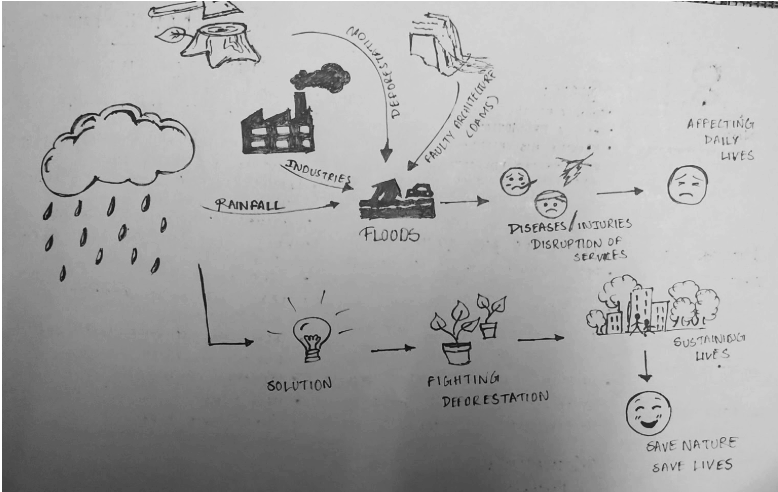
\includegraphics[width=\linewidth]{journeymap.png}
	\caption{Journey Map from adverse effects of floods \& deforestation to a greener and sustainable future.}
	\label{fig:map}
\end{figure}

Figure \ref{fig:map}

We will use statistical data based on various factors, maps and images. The datasets can either be real-time data collected from Synthetic Aperture Radar(SAR) or historical data recorded before.   

	\section*{Feasibility:}
		The risk of coastal flooding is increasing as a result of deforestation, untimely and torrential rains, sea level rise etc. In the event of floods occurring, a large amount of damage can be curbed if we have a model that could predict floods in advance. To avoid devastating consequences which have a major impact on economic and financial conditions of the city, our system aims to provide maximum accuracy in alerting target regions about the forthcoming disasters. This model can be extended for different locations in the future.
Not many ways we use today for addressing environmental challenges employ evolving and proven technologies like Artificial Intelligence and Machine Learning visible in inaccurate results (e.g. erroneous weather predictions etc).  The methods which are currently being used to address floods and other environmental challenges have a high degree of uncertainty associated with them.
With a reliable flood prediction model in place, government authorities in the targeted regions will be alerted about the impending floods in advance and will hence be able to evacuate the people living there and minimize other damages caused by the floods. Information regarding the range of the region which will be affected will enable the authorities to employ relief procedures accordingly.



\end{document}